\documentclass[a4paper,conference]{IEEEtran}
\IEEEoverridecommandlockouts
\usepackage{graphicx}
\usepackage{booktabs}
\usepackage{multirow}
\usepackage{cite}
\usepackage{url}
\usepackage{amsmath}

\title{Routing Errors Matter: A Lightweight Conditional Hierarchy for
Dermoscopic Skin Lesion Classification}

\author{\IEEEauthorblockN{Anonymous Authors}}

\begin{document}
\maketitle

\begin{abstract}
Flat multiclass classifiers conceal where errors arise, whereas conditional
hierarchies expose screening and subtype decisions but can propagate routing
errors. We compare a two-stage conditional hierarchy with a flat four-class
classifier using EfficientNet-B0 and the same locked, leakage-aware ISIC 2019
internal-test cohort of 3,668 dermoscopic images. The hierarchy first separates
non-malignant from malignant lesions and then conditionally classifies melanoma,
basal cell carcinoma, or squamous cell carcinoma. Its accuracy and macro-F1
were 0.740 and 0.605, compared with 0.742 and 0.619 for the flat model. The
paired flat-minus-hierarchical macro-F1 difference was 0.014 (95\% bootstrap
confidence interval: $-0.014$ to 0.042), and exact McNemar testing did not
detect a paired-correctness difference ($p=0.821$). With oracle routing,
hierarchical macro-F1 rose to 0.794, revealing a 0.188 routing-related loss;
20.08\% of malignant lesions were blocked at the first stage. A separate
five-class melanoma T-category feasibility experiment achieved macro-F1 0.276,
with zero recall for T2 and T4. Thus, overall performance was not statistically
distinguishable on this split, while routing error was the hierarchy's main
measured limitation and rare T-categories remained inadequately learned.
\end{abstract}

\begin{IEEEkeywords}
dermoscopy, hierarchical classification, skin lesions, routing error,
class imbalance, EfficientNet
\end{IEEEkeywords}

\section{Introduction}
Deep neural networks have enabled strong image-based skin-lesion classifiers
\cite{esteva2017,tschandl2020}, aided by public dermoscopic collections such as
HAM10000 \cite{tschandl2018} and ISIC challenges \cite{codella2019}. Most
systems nevertheless make one flat multiclass decision. A hierarchy can instead
represent a clinically meaningful coarse-to-fine decision, but a lesion sent
down the wrong branch cannot be recovered by a downstream classifier.

This work studies that failure mode without claiming clinical utility. Its
contributions are: (1) a fair same-split comparison of flat and conditional
hierarchical EfficientNet-B0 classifiers; (2) paired analysis of their overall
performance; (3) oracle-routing decomposition of loss caused by error
propagation; and (4) a separately reported melanoma T-category feasibility
study under severe label scarcity. We ask whether the hierarchy changes
four-class performance and, more importantly, how much of its loss is
attributable to routing.

\section{Related Work}
EfficientNet scales network depth, width, and resolution jointly and offers a
compact transfer-learning backbone \cite{tan2019}. Dermoscopic studies have
used deep ensembles and metadata to address heterogeneous lesion appearance
\cite{gessert2020}; controlled reader studies also show why evaluation design
and population scope matter \cite{tschandl2020}.

Hierarchical prediction incorporates label structure rather than treating all
errors identically. Barata \emph{et al.} combined a lesion hierarchy with
attention \cite{barata2019}, while hierarchical medical-image classifiers have
stacked models for coarse and fine decisions \cite{kowsari2020}. Such
factorization creates an error-propagation risk that headline accuracy alone
does not reveal. For imbalance, focal loss downweights easy examples
\cite{lin2017}, and effective-number weighting accounts for diminishing
information from repeated samples \cite{cui2019}. We combine these ideas only
in the malignant-subtype stage and focus on measured routing effects rather
than superiority claims.

\section{Materials and Methods}
\subsection{Dataset and Leakage-Aware Split}
We used the public ISIC 2019 training collection, whose sources include
HAM10000 and other multi-institutional dermoscopic sets
\cite{tschandl2018,combalia2019}. Diagnoses were mapped to four classes in the
fixed order: non-malignant, melanoma, basal cell carcinoma (BCC), and squamous
cell carcinoma (SCC). The seed-42 split was frozen before evaluation. Images
sharing a lesion identifier or exact file hash were assigned as connected
components; records without lesion identifiers used exact-hash grouping when
duplicated and otherwise remained singletons. The resulting train,
validation, and internal-test sizes were 17,124, 3,668, and 3,668. ISIC 2019
metadata did not provide patient identifiers, so patient-independent splitting
could not be guaranteed. Table~\ref{tab:setup} gives the class distribution.

\begin{table}[t]
\caption{Locked Four-Class Experimental Setup}
\label{tab:setup}
\centering
\setlength{\tabcolsep}{3.5pt}
\begin{tabular}{lrrr}
\toprule
Class & Train & Validation & Test\\
\midrule
Non-malignant & 11,193 & 2,398 & 2,398\\
Melanoma       & 3,164  & 678   & 678\\
BCC            & 2,327  & 498   & 498\\
SCC            & 440    & 94    & 94\\
\midrule
Total          & 17,124 & 3,668 & 3,668\\
\bottomrule
\end{tabular}
\end{table}

\subsection{Flat and Conditional Hierarchical Models}
Both designs used ImageNet-initialized EfficientNet-B0 \cite{tan2019}. The flat
model produced one four-class prediction. In the hierarchy (Fig.~\ref{fig:arch}),
Stage~1 classified non-malignant versus malignant. An argmax non-malignant
decision terminated inference; a malignant decision invoked Stage~2, which
classified melanoma, BCC, or SCC. This is a two-stage four-class system. The
later T-category study was not integrated into it.

\begin{figure}[t]
\centering
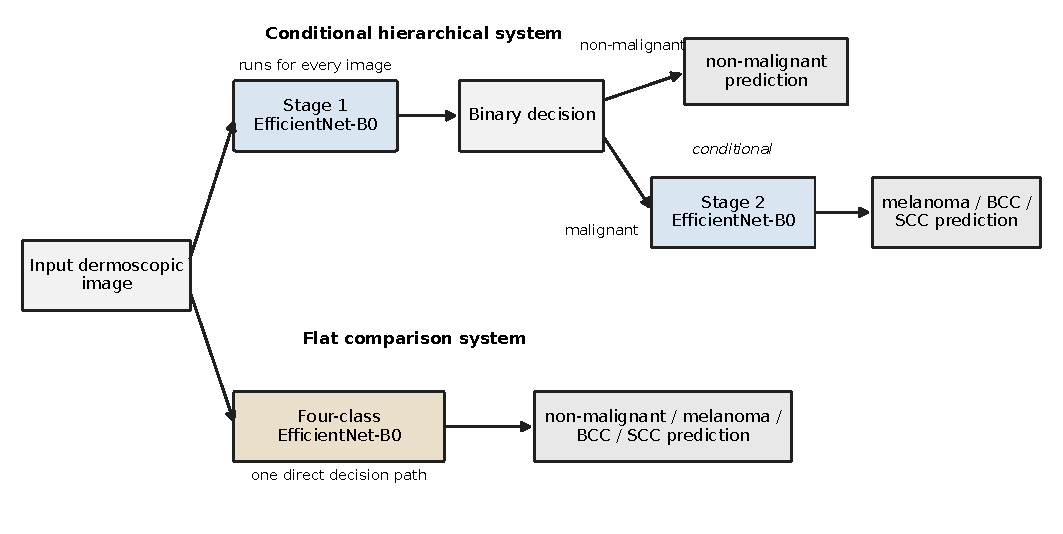
\includegraphics[width=\columnwidth]{figures/figure01_architecture.pdf}
\caption{Conditional hierarchical and flat architectures. Stage~1 runs for
every hierarchical input; Stage~2 is conditional on the malignant route.}
\label{fig:arch}
\end{figure}

\subsection{Training and Evaluation}
Images were ImageNet-normalized; evaluation resized the shorter side to 256
pixels and center-cropped to $224\times224$. Moderate training augmentation was
fixed across the main comparison. Models were trained for at most 30 epochs
with AdamW (learning rate $3\times10^{-4}$, weight decay $10^{-4}$), cosine
annealing, mixed precision, batch size 64, and early stopping patience 7.
Checkpoints were selected only by validation macro-F1.

Stage~1 and the flat model used cross-entropy. Stage~2 used focal loss
\cite{lin2017} with $\gamma=2$ and effective-number class weights
\cite{cui2019} computed on its training subset ($\beta=0.9999$). Each selected
checkpoint was evaluated once on the locked test split. We report accuracy,
balanced accuracy, macro-F1, and class F1; macro-F1 is primary because SCC is
rare.

\subsection{Routing and Statistical Analysis}
Predictions were paired by image identifier. A ground-truth-class-stratified
paired bootstrap (10,000 replicates, seed 42, percentile 95\% intervals)
preserved class support and estimated flat-minus-hierarchical differences. An
exact two-sided McNemar test used the discordant correctness pairs. An interval
including zero is interpreted as failure to establish a statistically
distinguishable difference, not equivalence or non-inferiority.

For diagnostic decomposition, oracle gating used the true
non-malignant/malignant label while retaining Stage~2 predictions. Its gap from
predicted gating quantifies routing-related loss, although the oracle is not a
deployable system.

\section{Results}
\subsection{Main Four-Class Comparison}
Table~\ref{tab:main} shows similar point estimates. Flat minus hierarchical
macro-F1 was 0.013855 (95\% CI: $-0.014255$, 0.041963); accuracy difference
was 0.001908 (95\% CI: $-0.011996$, 0.015812). The flat model alone was correct
on 354 images and the hierarchy alone on 347; exact McNemar $p=0.820742$.
Therefore, neither paired analysis established an overall difference on this
split.

\begin{table}[t]
\caption{Main Comparison on the Same 3,668 Images}
\label{tab:main}
\centering
\setlength{\tabcolsep}{3.1pt}
\begin{tabular}{lcccc}
\toprule
Model & Acc. & Bal. acc. & Macro-F1 & Weighted-F1\\
\midrule
Flat & 0.7421 & 0.6503 & 0.6192 & 0.7526\\
Hierarchy & 0.7402 & 0.6312 & 0.6054 & 0.7503\\
\midrule
Flat--hier. & 0.0019 & 0.0191 & 0.0139 & 0.0022\\
\bottomrule
\end{tabular}
\vspace{2pt}
\parbox{0.98\columnwidth}{\footnotesize Macro-F1 difference 95\% CI:
$[-0.0143,0.0420]$; exact McNemar $p=0.8207$.}
\end{table}

\begin{figure}[t]
\centering
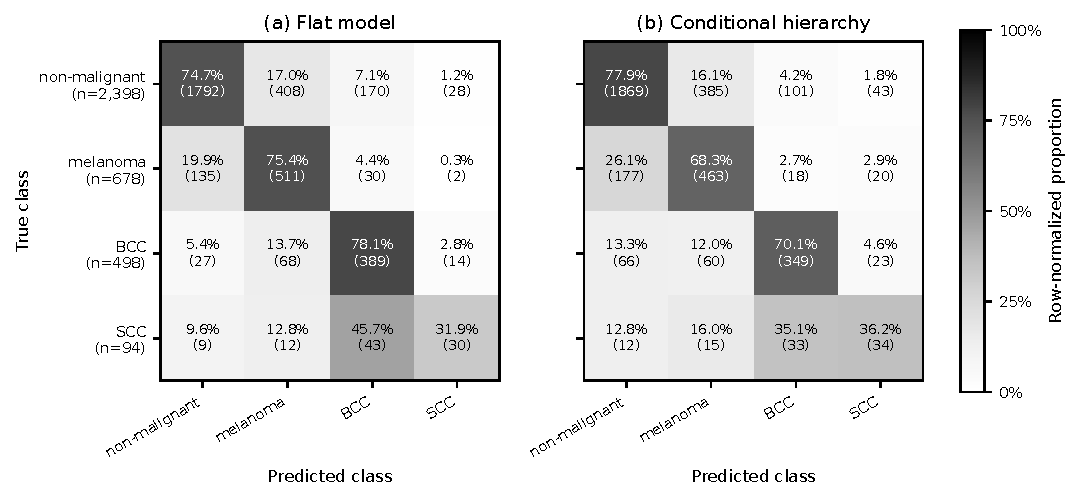
\includegraphics[width=\columnwidth]{figures/figure02_confusion_matrix_comparison.pdf}
\caption{Row-normalized confusion matrices on the locked test split. Rows are
true classes and columns predicted classes; cells also show raw counts.}
\label{fig:cm}
\end{figure}

\subsection{Routing-Error Decomposition}
With oracle routing, four-class macro-F1 was 0.793656 versus 0.605367 with the
predicted gate, an absolute loss of 0.188289 (Table~\ref{tab:routing}).
Stage~1 blocked 255 of 1,270 malignant images (20.079\%) and incorrectly sent
529 of 2,398 non-malignant images to Stage~2 (22.060\%). Among 1,015 correctly
routed malignant images, 169 (16.650\%) still received the wrong subtype.
Thus routing was the largest measured source of hierarchical loss, while
subtype discrimination remained a secondary limitation.

\subsection{Per-Class Behaviour}
Figure~\ref{fig:cm} displays the error distributions. Flat versus hierarchical
F1 was 0.822 versus 0.827 for non-malignant, 0.609 versus 0.578 for melanoma,
0.688 versus 0.699 for BCC, and 0.357 versus 0.318 for SCC. These comparisons
are exploratory: no class-wise hypothesis tests or multiplicity adjustment
were performed. SCC conclusions are especially unstable because support was
only 94.

\subsection{Standalone Stage-3 Feasibility}
A separate ISIC-derived melanoma subset contained 848 eligible images labelled
from official metadata into broad Tis, T1, T2, T3, and T4 categories. Known
patient, lesion, and exact-hash relations were kept within a seed-42
594/127/127 split. Two EfficientNet-B0 candidates differed only in loss and
were selected on validation macro-F1 before test access. The preselected
inverse-frequency weighted cross-entropy model obtained test macro-F1 0.275611
and balanced accuracy 0.386039 (ordinary cross-entropy: 0.162838 and
0.202403). T2 and T4 recall remained zero; their test supports were seven and
one. This experiment is feasibility evidence only, not clinical staging or an
evaluated third pipeline stage.

\begin{table}[t]
\caption{Routing Decomposition and Standalone Feasibility}
\label{tab:routing}
\centering
\setlength{\tabcolsep}{3.2pt}
\begin{tabular}{lrr}
\toprule
Quantity & Value & Denominator\\
\midrule
Oracle-gate macro-F1 & 0.7937 & 3,668\\
Predicted-gate macro-F1 & 0.6054 & 3,668\\
Routing-related loss & 0.1883 & ---\\
Malignant blocked & 20.079\% & 1,270\\
Non-malignant sent to Stage~2 & 22.060\% & 2,398\\
\midrule
Stage-3 weighted-CE macro-F1 & 0.2756 & 127\\
Stage-3 balanced accuracy & 0.3860 & 127\\
Stage-3 T2 / T4 recall & 0 / 0 & 7 / 1\\
\bottomrule
\end{tabular}
\end{table}

\section{Discussion and Limitations}
The hierarchy and flat comparator were not statistically distinguishable in
overall performance on this locked split. The oracle analysis adds information
that a flat comparison cannot: the hierarchy had a substantially higher
diagnostic ceiling, but Stage~1 errors prevented it from approaching that
ceiling. Improving the gate could therefore matter more than changing the
subtype model, although SCC remained difficult even after correct routing.

Several limitations constrain interpretation. Results come from one seed and
one internal ISIC 2019 split; no external evaluation was completed. Known
lesion and duplicate relations were leakage-controlled, but absent patient
identifiers prevent a guarantee of patient independence. The study did not
evaluate calibration, fairness across skin tones, explainability, clinical
workflow, latency, energy use, or deployment readiness. Bootstrap inference
conditions on the observed cohort, and a confidence interval containing zero
does not prove equivalence. Class-wise findings are exploratory, especially
for 94 SCC images. Finally, the T-category subset is small, highly imbalanced,
metadata-derived, and standalone; its rare-category results are inadequate and
it was never evaluated as part of a three-stage pipeline.

\section{Conclusion}
On the same locked 3,668-image cohort, flat and conditional hierarchical
EfficientNet-B0 classifiers had statistically indistinguishable overall
performance. Oracle gating exposed a 0.188 macro-F1 routing-related loss and a
20.08\% malignant blocking rate, identifying Stage~1 error propagation as the
hierarchy's main measured limitation. A separate T-category study further
showed that feasibility does not overcome severe rare-label scarcity. Future
work should validate routing improvements and the full system on independent
data before any clinical interpretation.

\bibliographystyle{IEEEtran}
\bibliography{references}
\end{document}
